\documentclass[a4paper]{article}
\usepackage{iwslt19,amssymb,amsmath,epsfig}
\setcounter{page}{1}
\sloppy		% better line breaks
%\ninept
%SM below a registered trademark definition
\def\reg{{\rm\ooalign{\hfil
     \raise.07ex\hbox{\scriptsize R}\hfil\crcr\mathhexbox20D}}}
\usepackage{amsmath,amsthm,amsfonts,amssymb,amscd}
\usepackage{graphicx}
\usepackage{multirow}
\usepackage{url}
\usepackage{float} 
\usepackage{tabularx}
\usepackage{xcolor}
\newtheorem{lemma}{Lemma}[section]
\newtheorem{theorem}{Theorem}[section]
\newtheorem{proposition}{Proposition}[section]
\newtheorem{definition}{Definition}[section]
\DeclareMathOperator*{\argmax}{argmax}
\DeclareMathOperator*{\argmin}{argmin}
\usepackage{algorithm}
\usepackage{algorithmic}
\usepackage[draft]{todo}

\floatname{algorithm}{Procedure}
\renewcommand{\algorithmicrequire}{\textbf{Input:}}
\renewcommand{\algorithmicensure}{\textbf{Output:}}
%\aclfinalcopy % Uncomment this line for the final submission
%\def\aclpaperid{***} %  Enter the acl Paper ID here

\newcommand{\fyTodo}[1]{\Todo[FY:]{\textcolor{orange}{#1}}}
\newcommand{\fyTodostar}[1]{\Todo*[FY:]{\textcolor{orange}{#1}}}
\newcommand{\fyDone}[1]{\done[FY]\Todo[FY:]{\textcolor{orange}{#1}}}
\newcommand{\fyDonestar}[1]{\done[FY]\Todo[FY:]{\textcolor{orange}{#1}}}
\newcommand{\jcTodo}[1]{\Todo[JC:]{\textcolor{orange}{#1}}}

%% \newcommand{\reg}{\textsuperscript{\textcircled{\textsc r}}}

\title{Lexicalized Domain Representations for Neural Machine Translation}

%%%%%%%%%%%%%%%%%%%%%%%%%%%%%%%%%%%%%%%%%%%%%%%%%%%%%%%%%%%%%%%%%%%%%%%%%%
%% Please make sure to keep technical paper submissions anonymous  !
%%%%%%%%%%%%%%%%%%%%%%%%%%%%%%%%%%%%%%%%%%%%%%%%%%%%%%%%%%%%%%%%%%%%%%%%%%
\name{Firstname Lastname}
%\name{MinhQuang Pham$^{\dag\ddag}$, \ Josep Crego$^\dag$, \ Fran\c cois Yvon$^\ddag$, \ Jean Senellart$^\dag$}

%%%%%%%%%%%%%%%%%%%%%%%%%%%%%%%%%%%%%%%%%%%%%%%%%%%%%%%%%%%%%%%%%%%%%%%%%%
%% If multiple authors, uncomment and edit the lines shown below.       %%
%% Note that each line must be emphasized {\em } by itself.             %%
%% (by Stephen Martucci, author of spconf.sty).                         %%
%%%%%%%%%%%%%%%%%%%%%%%%%%%%%%%%%%%%%%%%%%%%%%%%%%%%%%%%%%%%%%%%%%%%%%%%%%
% \makeatletter
% \def\name#1{\gdef\@name{#1\\}}
% \makeatother
% \name{{\em Firstname1 Lastname1, Firstname2 Lastname2, Firstname3 Lastname3,}\\
%      {\em Firstname4 Lastname4}}
%%%%%%%%%%%%%%% End of required multiple authors changes %%%%%%%%%%%%%%%%%

\address{ Affiliation / Address line 1 \\ Affiliation / Address line 2 \\ Affiliation / Address line 3 \\ {\small \tt email@domain}}
%\address{ $^\dag$SYSTRAN / 5 rue Feydeau, 75002 Paris, France \\ \small \tt firstname.lastname@systrangroup.com \\ $^\ddag$LIMSI, CNRS,  Universit\'e Paris-Saclay 91405 Orsay, France \\ {\small \tt firstname.lastname@limsi.fr}}

%
\begin{document}
\maketitle
%
\begin{abstract}
  Supervised machine translation works well when the train and test data are sampled from the same distribution.
  When this is not the case, \emph{adaptation} techniques help ensure that the knowledge learned from out-of-domain texts generalises to target domain sentences.
  We study here a related setting, \emph{multi-domain adaptation}, where the number of domains is potentially large and adapting separately to each domain would waste training resources.
  Our proposal transposes to neural machine translation the feature expansion technique of (Daum\'e III, 2007): it isolates domain-agnostic from domain-specific lexical representations, while sharing the rest of the network across domains.
  Our experiments use two neural architectures and two language pairs: they show that our approach, while remaining simple and computationally inexpensive, outperforms several strong baselines and delivers a multi-domain system that can successfully translate heterogeneous texts.
\end{abstract}

\section{Introduction \label{sec:introduction}}
Owing to the development of flexible and powerful architectures based on neural networks \cite{Cho14properties,Bahdanau15learning,Ghering17convolutional,Vaswani17attention}, 
Machine Translation (MT) has made significant progresses over the past years, and constitute to date the standard for most production engines. 
The development of MT systems, be they neural or statistical, require very large parallel corpora consisting of millions of sentence pairs, a resource that only exist in very few application domains and language pairs. 
A lot of the recent research effort has thus focused on developing MT systems in restricted data conditions, for instance building multilingual MTs which enable zero-shot translation \cite{Firat16multiway,Ha16towards,Johnson17google};
Another important scenario for industrial MT is to adapt a neural system trained using parallel data in one domain to the peculiarity of other domains. 

Domain Adaption (DA) in MT is an old issue \cite{Foster07mixture,Axelrod11domain}, which comes in various guises, and for which a number of solutions have been studied. 
See the recent survey of \cite{Chu18asurvey} for neural MT. 
The typical setting is \emph{supervised adaptation}, where a (small) amount of data of the target domain of interest is used to fine-tune the parameters of a system trained on a large amount of texts in a source domain. 
We study here a different scenario, \emph{multi-domain adaptation} \cite{Sennrich13multidomain,Farajian17multidomain}, where we would like to use heterogenous data sources to train a unique system that would work well for all domains. 
This allows us to be both data efficient (all data is used to train all domains) and computationally efficient (we only train one system).
Multi-domain adaptation is conceptually close to multilingual MT, or more generally to multi-task learning \cite{Caruana97multitask}, and can be approached in a number of ways. 

We adapt here ideas of \cite{Daume07frustratingly} to neural MT.
Our main hypothesis is that domains mostly differ at the lexical level, due to cross-domain polysemy, which motivates domain specific embeddings. 
By contrast, the deeper layers, which arguably model more abstract linguistic phenomena, are made shareable across domains. 
To this end, we design word embeddings containing a generic and several domain-specific regions. 
We experiment with three domains, two neural architectures and two language pairs and find that our technique yields effective multi-domain NMTs, outperforming several baselines. 
Our contributions are thus as follows:
we adapt and implement the ideas of \cite{Daume07frustratingly} for two NMT architectures;
we provide experimental evidence that show the effectiveness of this technique;
we evaluate the ability of our network to dynamically accommodate new domains;
and we introduce a novel technique to analyse word polysemy using word embeddings, which comforts the assumption that their variation across domains actually reflects a variation of senses.

\section{Lexicalized domain representations\label{sec:lexicalized_embeddings}}

\subsection{Multi-domain machine translation \label{ssec:statement}}

Multi-domain machine translation is formalized as follows: we assume observations taking the form of  domain-tagged sentence pairs $[(x,y),i]$, with $x$ in the source language, $y$ in the target language and $i$ a domain tag in $[1\dots d]$. We further assume a two-stage sampling process: first select a domain $i$ according to $p(i)$, then select a sentence pair according to a domain specific distribution $D_i$. Our objective is to find a tuple of parameters $\{\theta_1 \dots \theta_d \} \in \mathbb{R}^D \times \mathbb{R}^D \dots \times \mathbb{R}^D$ minimizing:
\begin{equation} \label{eq:loss}
\begin{split}
\sum_{i \in [1..d]} p(i) E_{(x,y) \sim D_{i}} [-log(p_{\theta_i}(y|x,i))]
\end{split}
\end{equation}
The training data for domain $i$ is denoted $C_i$.

A straightforward solution is to process each domain separately, computing the value $\theta_i^*$ that minimizes the empirical loss on $C_i$. This strategy is only effective if we have sufficient training data for each domain; when this is not the case, some estimates $\theta_i^*$ may be far from their optimal value. \fyDone{Risk}
The alternative we consider here constraints each parameter $\theta_i$ to be made of two parts: $\theta_i = [\theta_s; \theta'_i]$ ($\theta_s \in R^{D_g}$) is shared across all domains, while the second part $\theta'_i \in \mathbb{R}^{D_i}$ is only used in domain $i$.
The parameter set is now much more constrained, yet we expect that tying parameters across domains will yield better estimates for $\theta_s$ due to a larger training corpus. In this setting, the optimization program defined by equation~\eqref{eq:loss} can no longer be performed separately for each training corpus.

\subsection{Lexicalized domain embeddings \label{ssec:lde}}

To actually implement this idea for NMT, we need to define the subset of parameters that will be shared across domains. 
Our hypothesis is that domain specificities can be confined to the lexical level and define $\theta_s$ to contain all the network parameters except for a subpart of the word embeddings. 
For each word $v$, the embedding vector $e(v)$ is thus decomposed as $e(v) = [e_g(v); e_1(v); \dots; e_d(v)]$, where $e_g(v)$ stores the generic lexical embedding, while $e_i(v)$ stores the subpart that is specific to domain $i$.
In our NMT architectures, the actual embedding layer composes these vectors linearly to generate the word embedding for domain $k$ according to:

\begin{align}
  \tilde{e}_k(v) =& M_g e_g(v) + \sum_{i \in [1,..,d]} M_i * e_i(v) * \delta(i=k) \nonumber \\
   & = M [e_g(v); e_1'(v,k) \dots; e_d'(v,k)], \label{eq:embedding}
\end{align}
where $\delta()$ is the indicator function, $M$ is the matrix made of blocks $M_g, M_1 \dots, M_d$, and $e_i'(v,k)$ is the masked embedding: $e_i'(v,k)= e_i(v) * \delta(i=k)$.  

\begin{figure}[h]
  \center
  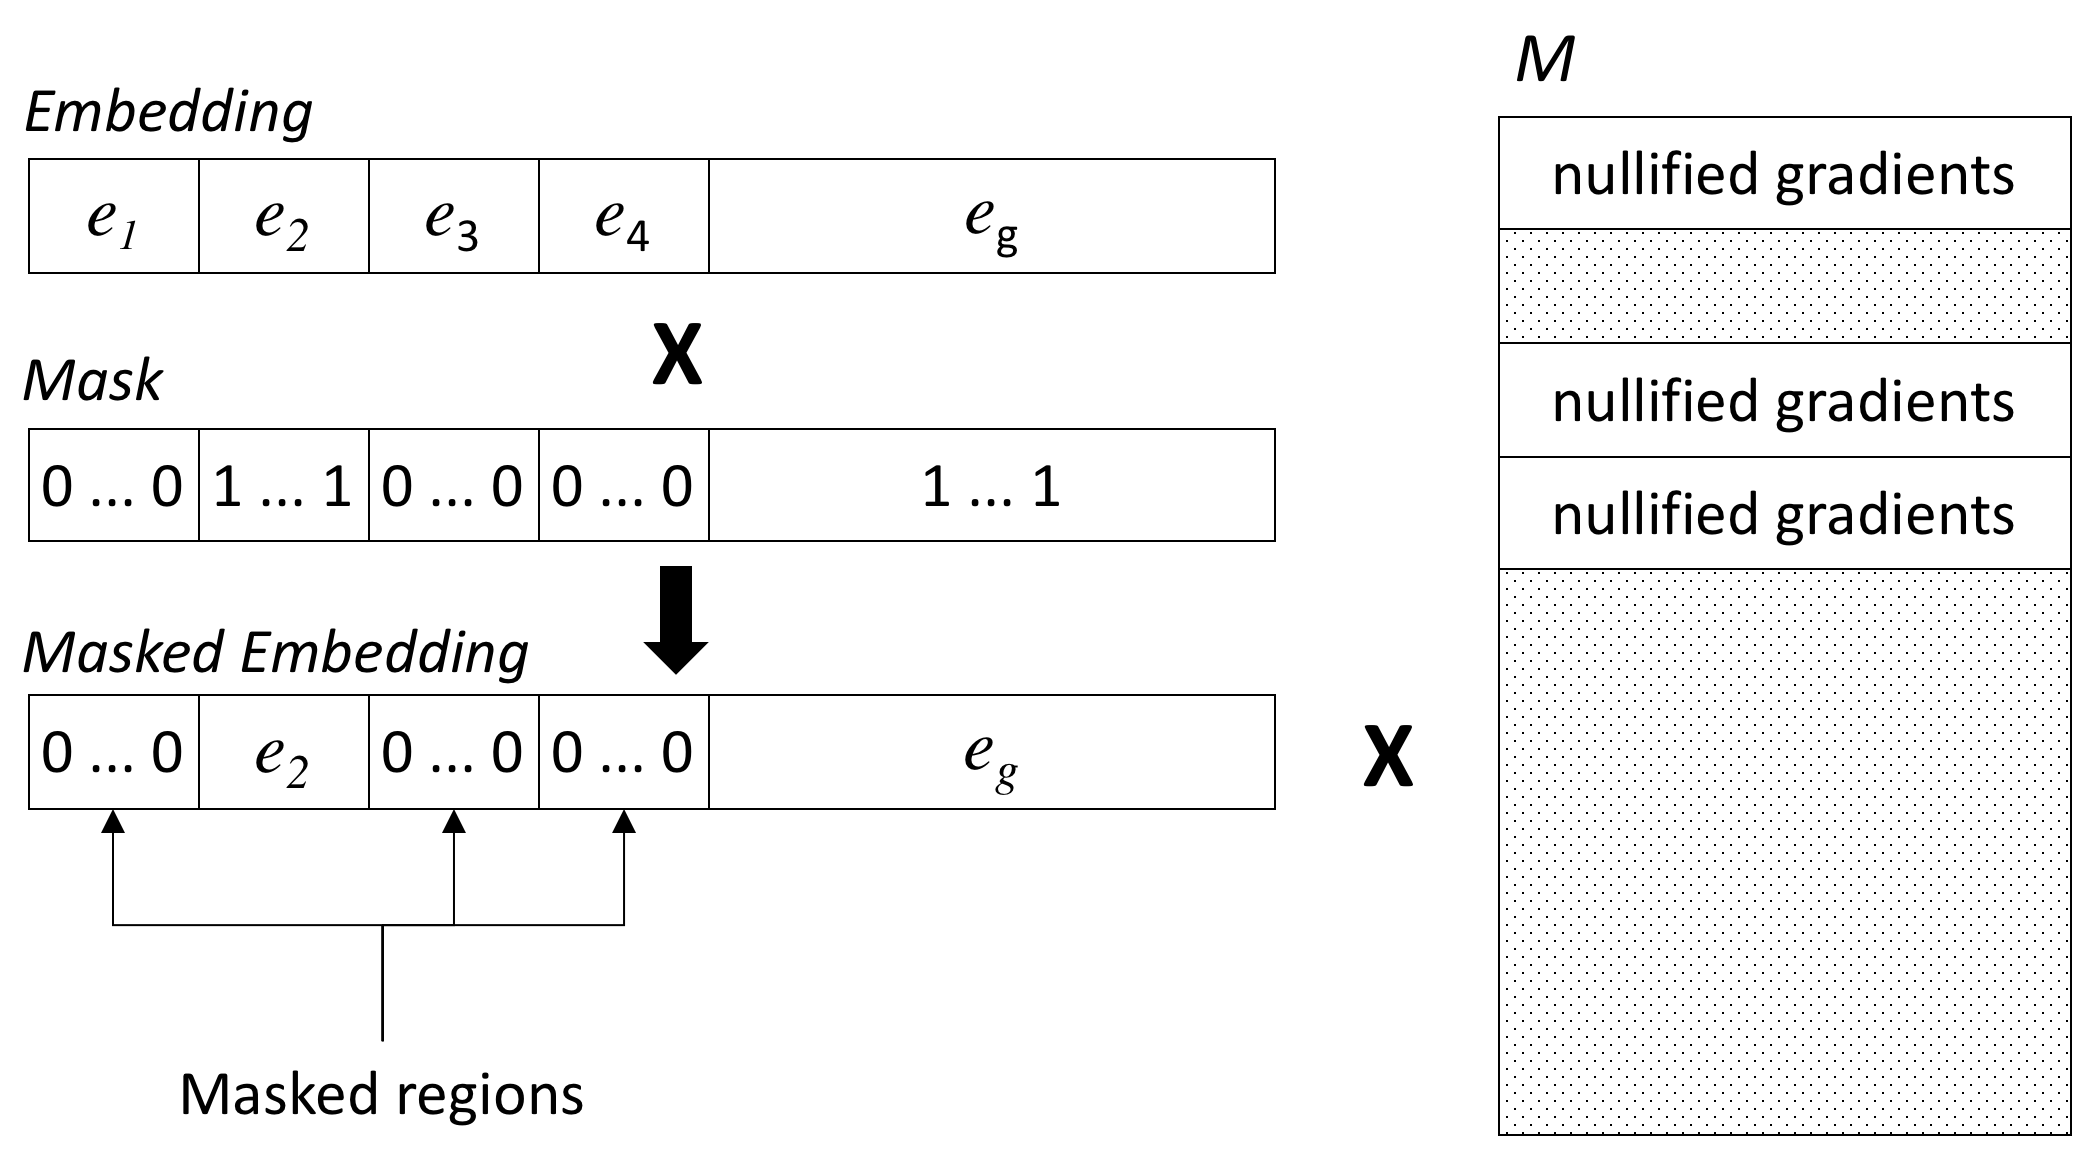
\includegraphics[width=0.48\textwidth]{embeddings}
  \caption{Lexicalized domain embeddings. When processing a sample from domain $2$, we only activate the corresponding parameter region ($\theta_2$) in the input embeddings; the remaining domain-specific parts are zeroed out, and do not receive any update. The generic part is always active and is updated irrespective of the input domain.} 
  \label{fig:network}
\end{figure}

Making sure that the actual embedding do not contain any zero is important for the Transformer model, since the lexical representations are then summed to the positional encoding, which would undo the effect of domain masking, and propagate a gradient even to regions that should not be modified. 
With our design, we make sure that during backprogation, the matrix $M$ receives gradient $0$ at regions corresponding to deactivated regions in the word embedding. 
Those regions are also masked in forward step, thus do not interfere the training on the domain to which they are not assigned (see Figure~\ref{fig:network}).
%
Our architecture is thus readily compatible with any NMT architecture, where we simply replace standard embedding layers the computation in equation~\eqref{eq:embedding}. In our experiments, we consider both the attentional RNN architecture of \cite{Bahdanau15learning} and for Transformer architecture of \cite{Vaswani17attention}.

% Let $\tilde{x}_{t} = M * e_{t} = M_g e_g(t) + \displaystyle{\mathop{\sum}_{i \in [1,..,d]} M_i * e_i(t)}$ be the projection of word embedding where $e_{t}$ is word embedding of token $x_{t}$, M is projection matrix, $M_j \forall j \in [1...d]$ is row block corresponding to domain region $j$ (Transformer \cite{Vaswani17attention}, recurrent \cite{Bahdanau15learning})\\
% Assume the batch belongs to domain $i$, then $e_j(t) = 0$ $\forall j \neq i$,$\forall t$. 
% \begin{equation}
% \begin{split}
% \frac{\partial L(x,y)}{\partial M_j} &= \sum_{t}\frac{\partial L}{\partial \tilde{x}_t}(x_t) * \frac{\partial \tilde{x}_t}{\partial M_j} \\
% 								&= \sum_{t} \frac{\partial L}{\partial \tilde{x}_t}(x_t) * e_j(t)\\
% 									&=0
% \end{split} 
% \forall j \neq i
% \end{equation}

% The complex structure of State-of-the-art architecture Transformer \cite{Vaswani17attention} and popular recurrent network \cite{Bahdanau15learning} makes the implementation of sparse embedding non-obvious. Indeed, Transformer involve positional embedding and residual connections which are not homogeneous for domain-regions. Therefore, in our first implementation, we used an dense layer to fuse domain-region and generic region before applying positional embedding and residual connection. This implementation limits the finetuning effect at only word level.\\
% Furthermore, because word embeddings are involved in three parts of standard encoder-decoder structure, which are input of encoder, input of decoder and projection before softmax, we have 7 possibilities to apply sparse embedding. However, due to high memory cost, we only want to apply sparse embedding on the source side. \fyTodo{Explain this. Future work ?}


% %%% 
% \fyTodo{Use math for notation, label equations and such}
% \begin{definition}{Domain}
% \label{def:domain}
% A domain is probabilistic distribution of translation $(x,y)$ in a given corpora. Given corpora $C$, we denote $D(C)$ the domain of $C$.
% \end{definition}
% \fyTodo{We need more: the source, the target, etc}
% In machine translation, the loss function for training is:
% \begin{equation}\label{eq:1}
% \begin{split}
% E_{(x,y) \sim p_{rel}}[-log(p_{\theta}(y|x))] &= \\
% = E_{x \sim p_{rel}(x)}[KL(p_{rel}(y|x) & \mid p_{\theta}(y|x))] + \\
% + E_{x \sim p_{rel}} &[H(p_{rel}(y|x))]
% \end{split}
% \end{equation}.

% Where $p_{\theta}(y|x) = p(y|x,\theta)$ \\
% In this equation, the domain is $p_{rel}(x,y)$. In minimizing given objective \ref{eq:1}, one aims to approximate the objective domain $p_{rel}$. In inference, provided the model was trained on certain training data, the more likely test set is generated from domain of training data, the better performance.\\
% In general, a generic model is trained first with a mix of several corpora which belongs to different topics (e.g medical, banking, adminstration) whose the domain $p_{rel}$ is considered as a general domain, noted $p_{gen}$. Being trained with a general mixed corpora, the generic model is not usually good enough for translating by topic. In order to improve topical translation quality, specializing generic model is required. One usually finetunes the generic model by continue the training from initial value $\theta^*$, which was optimized on general domain, using corpora of interested topic. However, there is always a dramatical shift from generic domain $p_{gen}$ to specialization domain $p_{spec}$. Indeed, the translation $(x,y)$ could be very different in different topic. For instance, in financial document, to translate "security" into "titre financier" is more likely than to translate it into "securit\'e" but in IT document. Therefore, the shift from general domain containing these two corpora to one of them is not negligible. This shift usually leads to catastrophic forgetting in neural network using backpropagation \cite{McCloskey1989Catastrophic}. In effect, the finetuned model usually shows lower performance in translating sentences, which are less related to the finetuning topic, than generic model. 
% In order to conduct the model translating topic by topic, we might refer to conditional probability conditioned by topic $p(y|x,d)$. Given a set of training corpora, we assume that there are a limited d engendering topic, i.e, there are d corpora $C_i$ $i \in [1,..,d]$ representing d topical domains $D(C_i)$ respectively. We are then interested in approximating $p(y,x|i)$ for $i \in [1,..,d]$ and use $p(y|x,i)$ for the inference in topic $i$. From now, we formalize the multi-domain problem for machine translation in following equation
% \begin{equation} \label{eq:2}
% \begin{split}
% \theta^* = \argmin_{\theta} \displaystyle{\mathop{\sum}_{i \in [1..d]}} E_{(x,y) \sim D(C_{i})}[-log(p_{\theta}(y|x,i))]
% \end{split}
% \end{equation}
% It is obvious that
% \begin{equation} \label{eq:3}
% \begin{split}
% \argmin_{\theta} \displaystyle{\mathop{\sum}_{i \in [1..d]}} E_{(x,y) \sim D(C_{i})} &[-log(p_{\theta}(y|x,i))] \\
% \geq \displaystyle{\mathop{\sum}_{i \in [1..d]}} \argmin_{\theta} E_{(x,y) \sim D(C_{i})} &[-log(p_{\theta}(y|x,i))]
% \end{split}
% \end{equation}
% A trivial solution for the equation \ref{eq:2} is $\theta^* = (\theta^*_{0},...,\theta^*_{d})$ and $p_{(\theta_{0},...,\theta_d)}(y|x,i)$ is independent of $\theta_{j}$ $\forall j \neq i$, i.e, $\exists f:\Omega_i \times C(D_i) \rightarrow [0,1]: f_{\theta_i}(y,x) = p_{(\theta_{0},...,\theta_d)}(y|x,i)$ where $\Omega_i$ is set of all possible values of $\theta_i$. \\
% The trivial solution is not rather than ensemble of $d$ models specialized for one domain. However, we could reduce the seperation by using shared paramaters denoted $\theta_s$ then reformulate the model as following: \\
% $\theta^* = (\theta^*_{0},...,\theta^*_{d}, \theta_s^*)$ and $p_{(\theta_{0},...,\theta_d, \theta_s)}(y|x,i)$ is independent of $\theta_{j}$ $\forall j \neq i$, i.e, $\exists f:\Omega_i \times \Omega_s \times C(D_i) \rightarrow [0,1]: f_{\theta_i, \theta_s}(y,x) = p_{(\theta_{0},...,\theta_d, \theta_s)}(y|x,i)$ \\ $p_{(\theta_{0},...,\theta_d, \theta_s)}(y|x)$ is independent of $\theta_{j}$ $\forall j$ i.e, $\exists \bar{f}:\Omega_s \times C \rightarrow [0,1]: \bar{f}_{\theta_s}(y,x) = p_{(\theta_{0},...,\theta_d, \theta_s)}(y|x)$
% where $\Omega_i$ is set of all possible values of $\theta_i$ and $\Omega_s$ is set of all possible values of $\theta_s$. The optimization problem will become
% \begin{equation}
% \displaystyle{\mathop{\sum}_{i \in [1..d]}} \argmin_{\theta_{0},...,\theta_{d}, \theta_s} E_{(x,y) \sim D(C_{i})} [-log(p_{\theta_s,\theta_i}(y|x,i))]
% \end{equation}
% However, the couple $\theta_s^*$ and $\theta_i^*$ are hardly optimal $\forall i \in [1..d]$.\\
% Despite the fact that $\theta^* = (\theta^*_{0},...,\theta^*_{d}, \theta_s^*)$ is hardly achieved by backpropagation, we could attempt to optimize $\theta_s$:
% \begin{equation}
% \theta^*_{s} = \displaystyle{\mathop{\argmin}_{\theta_s}}E_{(x,y) \sim D(\displaystyle{\mathop{\cup}_{i \in [1,..,d]}}C_{i})}[-log(p_{\theta_s}(y|x))]
% \end{equation} 

% then optimize each $\theta_i$ (as additional factor used for fine-tuning the model to the domain $D(C_{i})$) the perplexity with respect to true distribution of domain
% \begin{equation}
% \theta^*_{i} = \displaystyle{\mathop{\argmin}_{\theta_i}}E_{(x,y) \sim D(C_{i})}[-log(p_{\theta_i,\theta^*_s}(y|x,i))]
% \end{equation} 
% Our first approach to multi-domain machine translation is to build such trivial solution by assigning different regions of word embedding vector to set of domain paramters $\theta_i$ and set of shared parameters $\theta_s$ while keep sharing other parameters between domains.


\section{Experiments \label{sec:experiments}}

\subsection{Domains and data \label{ssec:data}}

We experiment with two language pairs (English-French, English-German) and data originated from three domains, corresponding to texts from three European institutions: 
the European Parlement (EPPS) \cite{Koehn05europarl}, 
the European Medicines Agency (EMEA), 
the European Central Bank (ECB) \cite{Tiedemann09news},
In addition, for English-French we also use IT-domain corpora obtained from the OPUS web site\footnote{\url{http://opus.nlpl.eu}} corresponding to KDE, Ubuntu, GNOME and PHP datasets (IT).
%
We randomly split those corpora into training, validation and test sets (see statistics in Table~\ref{tab:Corpora}).
Validation sets are used to chose the best model according to the average BLEU score \cite{Papineni02bleu}.
%Using internal test sets corresponds to somewhat ideal conditions.

%for contrast experiments, we also use supplementary test sets from three other domains: the official Khresmoi testset \cite{Khresmoi17test}, which is close to EMEA, News test 2014 \cite{Bojar14findings}, and IWSLT 2010 (Talk track) \cite{Paul10overview}. This enables us to evaluate the loss in performance when the test set is from a domain not seen in training.
% The model is also required to achieve comparable performance to generic model. To do so, we use newstest 2009 and IWSLT 2010 whose contain does not particularly belong to any domain.

\fyDone{Check which corpus are useful}
\begin{table}[h]
  \centering
  \begin{tabular}{ |llll|} %*{4}{|r|}}
    \hline
    Corpus & Train & Valid & Test \\ 
    \hline
    \multicolumn{4}{l}{English $\rightarrow$ French }\\
    %\multicolumn{4}{|l|}{Vocab size - En: 30,165, Fr: 30,398}\\
    \hline
    EMEA  & 1.09M & 1,000 & 1,000$_{300}$\\
    ECB    & 0.19M & 1,000 & 1,000     \\
    EPPS   & 2.01M  & 1,000 & 1,000  \\
    IT         & 0.54M  & 1,000 & 1,000 \\  
    \hline
    \multicolumn{4}{l}{English $\rightarrow$ German}\\
    %\multicolumn{4}{|l|}{Vocab size -  En:30,159, De: 30,698}\\ 
    \hline
    EMEA  & 1.11M & 1,000 & 1,000$_{300}$ \\
    ECB     &  0.11M & 1,000 & 1,000  \\
    EPPS   & 1.92M & 1,000 & 1,000 \\ 
    \hline
\end{tabular}
\caption{Corpora statistics.}
\label{tab:Corpora}
\end{table}

Note that the EMEA dataset as distributed on the OPUS site contains multiple sentence duplicates. 
We therefore report two numbers: the first is comparable to what has been published on earlier studies (eg.\ \cite{Zeng18multidomain}), the second one is obtained by making the test set entirely disjoint from the training set (700 duplicated sentences are discarded).

To reduce the number of lexical units and make our systems open-vocabulary, we apply Byte-Pair Encoding \cite{Sennrich16BPE} separately for each language with 30,000 merge operations. \fyDone{I need explanations here}

\subsection{Baselines \label{ssec:baselines}}
To validate our findings, we compared lexicalized domain embedding models with standard models using both attentional Recurrent Neural Networks (RNNs) \cite{Bahdanau15learning} and the Transformer architecture of \cite{Vaswani17attention}. Our baselines consist of:
\begin{itemize}
\item generic models trained with a simple concatenation of all corpora (\texttt{Mixed});
\item models tuned separately on each domain for respectively (10000, 15000, 5000) iterations using in-domain data (\texttt{ft$_{EMEA}$}, \texttt{ft$_{EPPS}$}, \texttt{ft$_{ECB}$}); 
\item models using domain tags as in \cite{Kobus17domaincontrol} (\texttt{DC}); 
\end{itemize}

For all models, we set the embeddings size equal to 512; the size of hidden layers is equal to 1024 for RNNs and 512 for Transformer. 
Other important configuration details are as follows:
Transformer models use multi-head attention with 8 heads in each of the 6 layers; 
the inner feedforward layer contains 2048 cells;  
RNN models use 1 layer on both sides: 
a bidirectional LSTM encoder and a unidirectional LSTM decoder with attention;
The domain control systems are exactly as their baseline counterparts (RNN and Transformer), with an additional 2 cells encoding the domain on the input layer.
 %
To train NMT systems, we use Adam, with parameters $\beta_1=0.9$, $\beta_2 = 0.999$, $\alpha=0.0005$ for RNNs; with parameters $\beta_1=0.9$, $\beta_2= 0.98$, with Noam decay \cite{Vaswani17attention} for Transformer ($warmup\_steps=4000$). In all cases, we use a batch size of~128 and a dropout rate of 0.1 for all layers. 
All our systems are implemented in OpenNMT-tf\footnote{\url{https://github.com/OpenNMT/OpenNMT-tf}} \cite{Klein17opennmt}

\subsection{Implementing Lexicalized Domain Representations}\fyDone{Check acronym.}

\fyDone{Motivate the split - discuss experimentally embedding size}
In order to implement lexicalised domain representations (henceforth \texttt{LDR}), we split the embedding vector into four regions: 
3 are domain specific and 1 is generic, with sizes $[8,8,8,488]$ respectively. %, a choice that will be discussed in Section~\ref{secc:region_size}. 
If a sentence originates from domain $i$, the domain specific regions for all domains $j \neq i$ will be zeroed out; while the other regions are activated (cf. Figure~\ref{fig:network}). 
We then use a dense layer of size~512 to fuse the region for the active domain and the ``generic'' region. Training is formalised in algorithm~\ref{alg:multidomain}.
%
Note that each iteration of algorithm \ref{alg:multidomain} uses 2~batches: a ``generic'' batch updating only the generic region; and a ``domain-specific'' batch updating just the domain-specific parameters. 

\begin{algorithm}[h]
\caption{Multi-domain Training}
\label{alg:multidomain}
\begin{algorithmic}[1]
\REQUIRE {Corpora $C_i, i\in [1,..,d]$ for $d$ domains, Batch size $B$}%, Optimization algorithm $\operatorname{Opt}$}
\REPEAT 
\STATE{Randomly pick $i \in [1,..,d]$ w.r.t the multinomial distribution $[\frac{|C_i|}{\sum_{i\in [1,..,d]}|C_i|}]$.}
\STATE{Randomly pick $B$ sentences from $C_i$.}
\STATE{Activate only generic region to create generic batch, denoted $W_g$.}
% \STATE{Pass the generic embedding batch to a dense layer.}
\STATE{Compute gradient of $\theta_s$, $\frac{\partial L}{\partial \theta_s}$ using $W_g$.}
\STATE{Activate domain-specific and generic regions to create domain-specific batch $W_i$}
% \STATE{Pass $W_i$ to a dense layer}
\STATE{Compute gradient of domain-specific parameters $\theta_i$, $\frac{\partial L}{\partial \theta_i}$ using $W_d$.}
\STATE{Update parameters $\theta_s$ using $\frac{\partial L}{\partial \theta_s}(W_g)$ and $\theta_i$ using $\frac{\partial L}{\partial \theta_i}(W_i)$}
% $$ \theta_s = \theta_s - \operatorname{Opt}(\frac{\partial L}{\partial \theta_s}(W_g))$$ 
% $$ \theta_i = \theta_i - \operatorname{Opt} (\frac{\partial L}{\partial \theta_i}(W_i))$$}
\UNTIL{convergence}
\end{algorithmic}
\end{algorithm}


The batch selection procedure (step~2 of algorithm~\ref{alg:multidomain}) ensures that the number of examples of each domain used in training  follows the distribution of the training data.
%each domain is represented according to its frequency in the training data. 
In our experiments, this means that sentences from the Europarl domain will be selected more frequently that the two other domains. In an attempt to build a more balanced training sample, we also consider an alternative selection procedure, where $i$ is selected according to  distribution $[\frac{\sqrt{|C_i|}}{\sum_{i\in [1,..,d]}\sqrt{|C_i|}}]$.

\subsection{Results \label{ssec:results}}

Results are summarized respectively in Table~\ref{tab:results-trsf} for the Transformer systems and Table~\ref{tab:results-rnn} for the RNN systems, where we report BLEU~\cite{Papineni02bleu} scores computed after detokenization.\footnote{As explained above, we  report two numbers when testing with EMEA, except for the fine-tuning scenarios when tuning on ECB and EPPS.} % \fyTodo{Footnote for missing numbers}.

%We first concentrate on the left part of these tables, where we analyze the performance for the three domains of interest. 
First, we observe that Transformer is consistently better than RNNs and that fine-tuning on a domain-specific corpus, when applicable, is almost the best way to optimize the performance on that domain.\footnote{This is not so clear for EPPS, where fine-tuning does not seem to help.}  
Note that fine-tuning will however yield a marked (even sometimes catastrophic, eg.\ for the EMEA-tuned Transformer system) decrease in performance for the other domains. 

Our approach (\texttt{LDR}$_{oracle}$) is consistently better than the \texttt{Mixed} strategy, with gains that range from very large (for EMEA and ECB) to unsignificant (for EPPS in most conditions). 
This means that our architecture is somehow able to compensate for the data unbalance and to raise the performance of the multi-domain system close to the best (fine-tuned) system in each domain. 
We even observe rare cases where the \texttt{LDR}$_{oracle}$ system outperforms fine-tuning (eg.\ Transformer en:de in the EMEA domain). 
\texttt{LDR}$_{oracle}$ is also better than Domain Control in three conditions out of four, \texttt{DC} being seemingly a better choice for the RNN than for the Transformer architecture. 
As expected, ignoring the true domain label yields a light drop in performance. %for the two fallback strategies considered in this study. 
%The first, \texttt{LDR}$_{generic}$, only uses the generic part of the embeddings. 
%The second, 
\texttt{LDR}$_{pred}$ employs automatically predicted domain labels.\footnote{Our domain classifier uses a bi-LSTM RNN encoder, followed by a simple softmax layer. 
Its precision on a development set exceeds 95\%.}
% \fyDone{Explain how}
Note that this decrease is however hardly significant, showing that our architecture is quite robust to noisy labels. 
Even in the worst case scenario where all domain tags are intentionally wrong (\texttt{LDR}$_{wrong}$), we see that the generic part still ensures a satisfying level of performance. 
A last contrast is with \texttt{LDR}$_{oracle}^{0.5}$ where we change the distribution of training sentences to decrease the weight of EPPS data and increase the number of ECB samples. 
As a result, we see a small decrease for EMEA and EPPS, and a large boost for ECB. 
This shows that our technique can be used in conjunction to other well known strategies for performing domain adaptation. 


% \fyTodo{Comment V2 from Minh}

%The right parts of Tables~\ref{tab:results-trsf} and \ref{tab:results-rnn} report performance on test sets for new domains not seen in training. 
%Khresmoi texts, which are extracted from summaries of medical articles are assumed to be from the same domain as EMEA data; 
%for the other two test sets, we assume no domain and only use the generic part of the embeddings. 
%Here, we see that our best system \texttt{LDR}$_{oracle}$ is slightly lagging behind the \texttt{Mixed} baselines (the difference ranges from unsignificant to one Bleu point), which can be attributed to larger useful (generic) embeddings in the \texttt{Mixed} setting. 
%Here again, we see that using the sole generic part makes the system robust with respect to unknown or misleading domain tags. 
%We finally outline that our approach outperforms DC for these test sets (were we have to commit to a predicted domain tag), and even outperforms WDCMT (for German-English). 
%This might be due to the fact that WDCMT has no built-in mechanism to ignore, as we do in the \texttt{LDR}$_{generic}$ systems, the possibly misleading predicted domain information.
\jcTodo{compute averages on all tables}

\begin{table}[!h]
\begin{center}
\scalebox{1.0}{
\begin{tabular}{|l|lcc|c|}
\hline
Model & EMEA & EPPS & ECB & Avg. \\
\hline
%\multicolumn{8}{l}{} \\[-9pt]  
\multicolumn{5}{l}{English$\rightarrow$French} \\
\hline
$\mathtt{Mixed}$          & 67.69$_{47.60}$ & 37.50 & 53.49 & \\
\hline
$\mathtt{FT}_{EMEA}$ & 76.77$_{49.43}$ & 17.16 & 11.99 &\\
$\mathtt{FT}_{EPPS}$  & 20.86 & 37.04 & 24.53 &  \\
$\mathtt{FT}_{ECB}$    & 26.93 & 27.09 & 56.52 & \\
\hline
$\mathtt{DC}$              & 67.87$_{45.42}$ & 37.31 & 54.14 & \\
\hline
$\mathtt{LDR}_{oracle}$            & 74.26$_{49.90}$ & 37.67 & 54.07 & \\
$\mathtt{LDR}_{oracle}^{0.5}$   & 74.95$_{49.38}$ & 37.35 & 55.91 & \\
%$\mathtt{LDR}_{generic}$          & 73.97$_{49.54}$ & 37.81 & 53.67 & \\
$\mathtt{LDR}_{pred}$               & 74.29$_{49.84}$ & 37.73 & 54.01 & \\
$\mathtt{LDR}_{wrong}$            & 72.95$_{49.78}$ & 37.62 & 53.35 & \\
  \hline
%\multicolumn{8}{l}{} \\[-9pt]
\multicolumn{5}{l}{English$\rightarrow$German} \\
\hline
$\mathtt{Mixed}$         & 64.57$_{42.99}$ & 26.47 & 68.67 & \\
\hline
$\mathtt{FT}_{EMEA}$ & 68.35$_{42.97}$ & 17.02 & 32.87 & \\
$\mathtt{FT}_{EPPS}$  & 36.19 & 26.29 & 40.71 & \\
$\mathtt{FT}_{ECB}$   & 24.72 & 18.36 & 74.05 & \\
\hline
$\mathtt{DC}$ & 63.48$_{42.98}$ & 26.27 & 66.95 & \\
\hline
$\mathtt{LDR}_{oracle}$ & 70.90$_{46.12}$ & 26.30 & 68.90 & \\
$\mathtt{LDR}_{oracle}^{0.5}$ & 71.31$_{45.23}$ & 25.98 & 73.74 & \\
%$\mathtt{LDR}_{generic}$ & 70.86$_{45.60}$ & 26.14 & 68.59 & \\
$\mathtt{LDR}_{pred}$ & 70.89$_{46.12}$ & 26.53 & 68.63 & \\
$\mathtt{LDR}_{wrong}$ & 69.51$_{43.50}$ & 26.31 & 66.86 & \\
\hline
\end{tabular}
} %scalebox
\end{center}
\caption{BLEU scores for  Transformer systems \label{tab:results-trsf}}
\end{table}




\begin{table}[!h]
\begin{center}
\scalebox{1.0}{
\begin{tabular}{|l|lcc|c|}
\hline
Model & EMEA & EPPS & ECB & Avg. \\
\hline
%\multicolumn{8}{l}{} \\[-9pt]
\multicolumn{5}{l}{English$\rightarrow$French} \\
\hline
$Mixed$                         & 65.42$_{45.11}$ & 34.70 & 51.38 & \\
\hline
$\mathtt{FT}_{EMEA}$   & 72.06$_{47.33}$ & 18.62 & 16.78 & \\
$\mathtt{FT}_{EPPS}$    & 35.47$ $ & 34.61 & 39.56 & \\
$\mathtt{FT}_{ECB}$      & 21.93$ $ & 22.60 & 51.53 & \\
\hline
$\mathtt{DC}$                            & 68.26$_{43.76}$ & 35.13 & 50.09 & \\
% \hline
%$\mathtt{WDCMT}$           & 68.76$_{45.29}$ & 35.71 & 52.75 & \\
\hline
$\mathtt{LDR}_{oracle}$            & 71.73$_{46.30}$ & 35.21 & 50.91 & \\
%$\mathtt{LDR_{condgru}}_{pred}$   & 71.7$_{46.21}$ & 35.09 & 51.22 & \\
$\mathtt{LDR}_{oracle}^{0.5}$   & 71.70$_{46.41}$ & 34.24& 52.37 & \\
%$\mathtt{LDR}_{generic}$          & 70.59$_{46.37}$ & 35.22 & 49.68 & \\
$\mathtt{LDR}_{pred}$               & 72.76$_{46.35}$ & 35.10 & 50.38 & \\
$\mathtt{LDR}_{wrong}$            & 62.10$_{43.29}$ & 34.17 & 48.79 & \\
\hline
%\multicolumn{8}{l}{} \\[-9pt]
\multicolumn{5}{l}{English$\rightarrow$German} \\
\hline
$Mixed$                        & 57.37$_{37.94}$ & 23.10 & 63.54 & \\
\hline
$\mathtt{FT}_{EMEA}$  & 65.64$_{44.71}$ & 12.36 & 15.93 & \\
$\mathtt{FT}_{EPPS}$   & 24.90$ $ & 22.98 & 26.26 & \\
$\mathtt{FT}_{ECB}$     & 41.80$ $ & 15.97 & 71.07 & \\
\hline
$\mathtt{DC}$                & 62.53$_{39.25}$ & 23.74 & 65.71 & \\
%\hline
%$\mathtt{WDCMT}$ & 64.05$_{38.54}$ & 22.82 & 67.00 & \\
\hline
$\mathtt{LDR}_{oracle}$     & 63.43$_{40.04}$ & 22.66 & 64.40 & \\
$\mathtt{LDR}_{oracle}^{0.5}$   & 63.27$_{38.16}$ & 21.83 & 69.55 & \\
%$\mathtt{LDR}_{generic}$   & 63.27 $_{39.75}$ & 22.62 & 63.70 & \\
$\mathtt{LDR}_{pred}$        & 63.17$_{39.92}$ & 22.51 & 64.00 & \\
$\mathtt{LDR}_{wrong}$     & 56.84$_{37.05}$ & 22.06 & 61.66 & \\
\hline
\end{tabular}
} %scalebox
\end{center}
\caption{BLEU scores for RNN systems\label{tab:results-rnn}}
\end{table}
% \clearfloat

We also compare our architecture with the multi-domain model of \cite{Zeng18multidomain} (\texttt{WDCMT}) for the pair English$\rightarrow$French. We use the author's implementation\footnote{\noindent\url{http://github.com/DeepLearnXMU/WDCNMT}} that is composed of one bidirectional Gated recurrent units (GRU) layer on the encoder side; and one unidirectional conditional GRU layer on the decoder side; the dimension of ``domain'' layers is~300.
%
The direct comparison with our RNN is difficult, as both networks differ in many ways: framework, cell types, \textit{etc.}. The results in Table~\ref{tab:results-rnn-wdcmt} therefore use a variant of our model that makes it more similar to that of the \texttt{WDCMT} network. In particular, this variant also uses a single GRU layer in the encoder and a single conditional GRU layer in the decoder ($\mathtt{LDR}_{pred}^{condgru}$). As can be seen in this table, our model is on average comparable to \texttt{WDCMT}, while using a much simpler design.
%However, the comparison with \texttt{WDCMT} is difficult as the implementation differs in many ways from our RNN: framework, cell types,  etc.
%Thus, in order to compare closer architectures we replace our model to use a single GRU layer in the encoder and a decoder with a single conditional GRU layer ($\mathtt{LDR}_{pred}^{condgru}$).
%
% Results are shown by Table~\ref{tab:results-rnn-wdcmt}.
% The comparison is less favourable for our RNN system, which is arguably much simpler.

\begin{table}[!h]
\begin{center}
\scalebox{1.0}{
\begin{tabular}{|l|ccc|c|}
\hline
Model & EMEA & EPPS & ECB & Avg. \\
\hline
%\multicolumn{8}{l}{} \\[-9pt]
\multicolumn{5}{l}{English$\rightarrow$French} \\
\hline
$\mathtt{LDR}_{pred}$               & 72.76$_{46.35}$ & 35.10 & 50.38 & \\
$\mathtt{LDR}_{pred}^{condgru}$  & 71.70$_{46.21}$ & 35.09 & 51.22 & \\
$\mathtt{WDCMT}$                  & 68.76$_{45.29}$ & 35.71 & 52.75 & \\
\hline
\end{tabular}
} %scalebox
\end{center}
\caption{BLEU scores for RNN systems. Comparison between \texttt{WDCMT} and $\texttt{LDR}_{pred}$ built using conditional GRUs.\label{tab:results-rnn-wdcmt}}
\end{table}

\section{Complementary experiments\label{sec:Discussion}}

% \subsection{Sparse's performance}
% First, we analyze the performance of models on inner test sets which are created by randomly splited from same corpora as training set. The 4 table show remarquable improvement 6 points BLEU in average in EMEA translation which is comparable with finetuned model. In all most the cases, Sparse model has slightly higher score on EPPS test and ECB test than mixed and finetuned models. Sparse model also achieve comparable scores with Domain Control and WDCMT in average. In considering the score of finetuned model on out-of-domain test sets, we observed a fast catastrophic forgetting while the out-of-domain scores drop dramatically compared to mixed model. Taking into account the average score on 3 inner test sets, Sparse achieved far better score than all finetuned models. \\
% Secondly, we compare performance of models on IWSLT test 2010 and newstest 2014 which are more general than inner test sets. On these test sets, mixed, Sparse has approximately same score in Transformer and are a little better than Domain Control while in Recurrent Net Work architecture, WDCMT is better than mixed, Sparse and Domain Control for English -French pair. We also noted a quick fall of performance in finetuned model.

\subsection{Balancing generic and domain representations\label{secc:region_size}}

An important practical question concerns the balance between the generic and the domain-specific part of the embeddings. 
In the limit where the domain specific part is very small, we should recover the performance of the \texttt{Mixed} system; 
conversely, we expect to see a less effective sharing of data across domains by increasing the domain-specific regions. 
Table~\ref{tab:embedding-size} reports the result of  a series of experiments for the Transformer architecture (English-French) with varying domain-specific sizes allocating between 4 and 64 cells for domain-specific information, and the complement to 512 for the generic part. 
The differences are overall quite small in our experimental setting, where the training data is relatively limited and does not require to use a large embedding size. 
We therefore decided to allocate $8$~cells for the domain specific part. 
This suggests that we could easily accommodate more domains with the same architecture, and even reserve some regions to handle supplementary data. %incoming training data.  
% \fyTodo{Easily accomodate more domains}
\fyDone{Given the ways embeddings are computed, why not add more domains, and test robustness agains data presentation order ?}

\begin{table}[!h]
\begin{center}
\scalebox{1.0}{
\begin{tabular}{|l|ccc|c|}
\hline
$\mathtt{LDR}_{oracle}$ & EMEA & EPPS & ECB & Avg. \\
\hline
\multicolumn{5}{l}{English$\rightarrow$French} \\
\hline
 size=4   & 74.65$_{49.61}$ & 37.42 & 54.49 & \\
 size=8   & 74.26$_{49.90}$ & 37.67 & 54.07 & \\
 size=16 & 74.15$_{49.10}$ & 37.78 & 54.56 & \\
 size=32 & 75.10$_{48.61}$ & 37.64 & 54.29 & \\
 size=64 & 74.50$_{50.17}$ & 37.27 & 54.50 & \\
\hline
\end{tabular}
} %scalebox
\end{center}
\caption{BLEU scores for the Transformer architecture for varying domain-specific embedding sizes \label{tab:embedding-size}}
\end{table}

\subsection{Additional Domain Scenario \label{ssec:additiona_domain}}

We now evaluate the ability of our model to integrate new domains, a very common scenario for industrial MT. In this setting, we consider that we have a model ($\mathtt{LDR}_{oracle}$) trained as before for EMEA, EPPS and ECB during 200,000 iterations, which needs to accomodate new training data in the IT domain. Assuming that we have reserved extra empty embedding cells\footnote{For this experiment, word embeddings contain 480 cells for the generic region and 32 cells for domain specific regions (8 cells x 4 regions).} for this new domain, we resume training with 4 domains during 100,000 additional iterations, yielding a updated model  $\mathtt{LDR}_{oracle}^*$. Experiments are reported for the English$\rightarrow$French language pair in Table~\ref{tab:add}, where for comparison purposes we also report numbers obtained with continued training with the $\mathtt{Mixed}$ model, training for the same number of iterations and using the same four datasets ($\mathtt{Mixed}^*$).

\begin{table}[!h]
\begin{center}
\scalebox{0.9}{
\begin{tabular}{|l|cccc|c|}
\hline
Model & EMEA & EPPS & ECB & IT & Avg.\\
\hline
\multicolumn{5}{l}{English$\rightarrow$French} \\
\hline
$\mathtt{Mixed}$                & 67.69$_{47.60}$ & 37.50 & 53.49 & 13.91 & \\
$\mathtt{Mixed}^*$             & 66.49$_{45.79}$ & 37.59 & 55.07 & 51.78 & \\
\hline
$\mathtt{LDR}_{oracle}$     & 74.26$_{49.90}$ & 37.67 & 54.07 & 13.40 & \\
$\mathtt{LDR}_{oracle}^*$  & 76.17$_{49.71}$ & 37.48 & 55.12 & 55.24 & \\
\hline
\end{tabular}
} %scalebox
\end{center}
\caption{BLEU scores for the Transformer architecture when including IT as additional domain \label{tab:add}}
\end{table}

As expected, a huge improvement in performance is observed for the IT test set when learning includes in-domain data for both models, with$\mathtt{LDR}_{oracle}^*$ outperforming $\mathtt{Mixed}^*$ by a wide margin.
%
It is interesting to see that this additional data has also a positive impact on other test sets: both models similarly increase their performance for the ECB domain, and $\mathtt{LDR}_{oracle}^*$ additionally improves the results for the EMEA test, which is not the case for $\mathtt{Mixed}^*$;
finally, using IT data does not impact the quality of translations for the EPPS domain of any of the models. Overall better results are obtained by our $\mathtt{LDR}_{oracle}$ model when trained including the additional domain dataset, demonstrating the ability of the model to seamlessly integrate new domains. % as supplementary training data becomes available.
%New domains are easily integrated in the model if the corresponding embedding regions are reserved in advance.

\subsection{Analysis of Word Embeddings \label{ssec:word_embeddings}}
One of our main assumptions is that the difference between domains can be confined at the lexical level, warranting our decision to specialise lexical representations for each domain, while the remaining part of the network is shared across domains. Linguistically, this assumption relates to the classical ``one sense per collocation'' \cite{Yarowsky93onesense} and corresponds to the fact that in many cases, polysemy corresponds to variation of use across domain. In its weaker form, it allows us to assume that all occurrences of a given form in a given domain correspond to the same sense and share the same representation; the same form occurring in different domains is allowed to have one distinct embedding per domain, which may help capture polysemy and lexical ambiguity in translation. 

To check this hypothesis, we performed the following analysis of embeddings learned with the multi-domain Transformer system for English:French. For each unit\footnote{In this study, we work with BPE units, not words, meaning that in many cases we observe the variation of use of word parts. As we work with a large inventory, many of these units correspond to actual words, and we focus on these in our comments. We also restrict our analysis to words that occur at least 30 times in each domain, to ensure that each domain-specific region is updated during training.} in our English dictionary, we compute the $k$ nearest neighbours for each domain $i \in [1\dots{}d]$, where the distance between unit $u$ and $v$ for domain $i$ is the cosine distance in the corresponding embedding space, ie.\ assuming that the actual embedding of $v$ for domain $i$ is $e(v,i) = M_ge_g(u) + M_de_i(v)$ (cf.\ equation~\eqref{eq:embedding}). This process yields $d$ lists of $k$ nearest neighbours. The size of their intersection should then be a sign of a variation of use across domains; conversely, an identical set of neighbours across domains should reflect the stability of word use. Table~\ref{tab:embeddings} list the 10 units with the smaller (respectively larger) intersection (we use $k=10$ and $d=3$). 

\begin{table}[h]
  \centering
%  \begin{tabularx}{1.0\linewidth}{c|c}
  \begin{tabular}{c|c}
    Polysemic ``words'' & Monosemic ``words'' \\ \hline
     ases (0) &               obtain (10) \\       
     impairment (1) &     virtually (10) \\    
     convenience (1) &    represent (10) \\    
     oring (1) &              safety (10) \\       
     ums (1) &               defence (10) \\      
     turnover (1) &         coordinated (10) \\  
     occurrence (1) &     handling (10) \\     
     tent (2) &               July (10) \\         
     ture (2) &               previous (10) \\     
     mation (2) &           better (10) \\ \hline
  \end{tabular}
  \caption{Analyzing the variation of embeddings across domains. Each word or subword is listed with the size of the intersection (between 0 and 10).}
  \label{tab:embeddings}
\end{table}

Let us first consider the full words in the left column of Table~\ref{tab:embeddings}. The case of \emph{impairment} is pretty clear, occuring in EMEA mostly in terms such as ``hepatic impairment'' or ``renal impairment'', and translating into French as \textsl{insuffisance}. In ECB, its collocate are quite different, and impairment often occurs in terms such as ``cost subject to impairments'' (French: \emph{co\^ut soumis \`a des r\'eductions de valeur}). Likewise, ``convenience'' seems to have its general meaning (``for convenience'') in EMEA, but appears in ECB in the specific context of ``convenience credit card'' (French \textsl{carte de cr\' edit \`a remboursement diff\'er\'e}). We finally see the same phenomena with ``turnover'', which is consistently translated with its economic meaning (French \textsl{chiffre d'affaire}) in ECB and EPPS, but whose collocates in EMEA ("bone turnover", ``hepatic turnover'') are associated with the idea of the cell renewall process, yielding translations such as \textsl{remodelage osseux} in French. Subword units can be analysed in the same ways: ``ums'', for instance, appears in words such as ``gums'', ``serums'', ``vacuums''  in EMEA; in ECB, ``ums'' is mostly the suffix of ``maximums'', ``minimums'', or ``premiums''; EPPS finally contains a more diverse set of ``-ums'' ending words (``stadium'', ``forum'', equilibrium'', etc). 

Let us now consider the list of putative monosemic words (on the right part of Table~\ref{tab:embeddings}), ie.\ words for which the nearest neighbors are the same in all domains, contains mostly words for which we do not expect much variation in translation: adjective (``previous'', ``better''), adverbs (``virtually``), generic verbs (``handling'', ``coordinated''), etc; and the list of words having a constant set of neighbors also contains prepositions (``at'', ``in''), auxiliary (``been'') etc.  

\section{Related Work \label{sec:related_work}}
Domain adaptation (DA) is a vexing problem in NLP, which appears in a wide range of practical situations and data scenarios (eg.\ supervised vs. unsupervised adaptation), and  has been thoroughly  studied from a number of perspectives, ranging from theoretical analysis to more applied work, and for which many solutions have been proposed. The literature of DA for Machine Translation reflects this diversity and typically distinguishes data-based approaches from model-based approaches \cite{Chu2017comparison,Chu18asurvey}.

The most common adaptation scenario uses (mostly) out-of-domain data in training, while testing on a low-resource in-domain set of texts. In this setting, \emph{data-based approaches} aim to bias the distribution of the train (out-of-domain) data towards matching that of the target domain, using data selection techniques \cite{Moore10selection,Axelrod11domain,Duh13selection}, or generating adapted pseudo-parallel data through back-translation  \cite{Utiyama03measure,Wang14neural,Wang16connecting,Sennrich16improving}. \emph{Model-centric approaches} build domain-adapted models by combining (eg.\ with mixture weights) multiple data sources or multiple systems \cite{Foster07mixture,Wang17instance}, or by biasing the training objective towards the desired domain using in-domain adaptation data \cite{Luong15stanford,Freitag16fast,Chen17costweighting}. Another approach worth mentioning integrates domain information (for instance a domain language model) in the decoding algorithm \cite{Gulcehre17onintegrating}.
%
Our scenario is a bit different as we aim to train a unique system that will work well for several domains. This corresponds to a practical scenario in the industry, where one would like to maintain one single multi-domain engine, trained on all the available (heteregeneous) sources of data. Our primary source of inspiration is the proposal of \cite{Daume07frustratingly} who proposes to use several copies of the same features (one ``generic'' shared across domains, and one for each domain), letting the training adjust their respective weights. This work has been reanalyzed in a Bayesian framework in \cite{Finkel09hierarchical}, and revisited notably in \cite{Chang10necessity}. Following up on \cite{Yang15unified}, the recent proposals of \cite{Peng17multitask} apply the same idea with neural architectures, using domain specific masking to zero out the parameters modeling domains irrelevant to the current input sentence. Compared to our work, these techniques are used in deep network layers and applied to sequence labelling tasks.

The multi-domain scenario in NMT has been studied in a number of recent works. \cite{Farajian17multidomain} learn a generic system and propose to dynamically adapt the network weights in an unsupervised manner using a small sample of training data that resembles the test data, an idea already explored in \cite{Sennrich13multidomain}. Their main contribution is to propose an a method to relate the amount of adaptation of the network parameters to the similarity between the adaptation sample and the test sentence: the higher the similarity, the more agressive the adaptation.
%
By analogy with the proposal of \cite{Johnson17google} for multilingual NMT, \cite{Kobus17domaincontrol} and \cite{Chu18multilingual} separately propose to extend the representation of the source text with a domain tag. Our model also modifies input representations, but allows each source word to have a domain-specific representation, thereby improving training of the shared parts of the network.\fyDone{Talk about target embeddings somewhere.} 

Similarly to our approach, \cite{Zeng18multidomain} attempts to separate on the encoder side domain-specific representation from generic representations in two different sub-networks, where generic versus domain-specific representations automatically emerge from two adversarial networks. 
The decoder side can thus attend separately to these two representations to generate its output. 
In this approach, the shared and domain-specific part kept separated in the deeper layers of the network, whereas we try to localise the differences between domains at the lexical level, based on a much cheaper computational architecture. 
Another trait of this proposal is the ability to automatically infer domain information for test sentences; 
as we have shown, our architecture can also effectively accommodate sentences lacking domain information.

\section{Conclusions}
In this paper, we have presented a new technique for multi-domain machine translation,  adapting the ``frustratingly easy'' idea of \cite{Daume07frustratingly} to two standard NMT architectures. 
Our experiments have shown that for both architectures and for two language pairs, our multi-domain models improve over several baselines of the literature and that it is robust to noise in domain labels. It is noticeable that these results are obtained without impacting the architecture or training complexity
, making our approach a simple baseline for further studies in multi-domain translation
.
We have also shown that our approach can dynamically handle new domains; and that the domain-specific embeddings often reflect differences of senses. In our future work, we intend to develop these ideas so as to make the architecture more self-configurable and able to adapt the size of the domain-specific regions depending upon the actual variation of use across domains; we also would like to find additional ways to make the architecture able to integrate an arbitrary number of new domains in a dynamic fashion, as this is an important requirement in industrial systems.

%\section{Acknowledgements}
%The IWSLT 2015 organizing committee would like to thank the
%organizing committees of INTERSPEECH 2004 for their
%help and for kindly providing the template files.

%
\bibliography{iwslt19}
\bibliographystyle{IEEEtran}
\end{document}

